%
% This is Chapter 1 file (chap1.tex)
%
\chapter{Introduction}

\section{Problem Overview and Proposed Solutions}

Scientific simulations are increasingly being migrated to
extreme-scale platforms consisting of hundreds (or thousands) of
multicore servers equipped with many-core accelerators. The increasing
number of nodes and cores is resulting in an increasing level of
concurrency and ultimately non-determinism in the execution of large
scale applications on these platforms. Table~\ref{tab:trends} shows
the concurrency levels in 2010 and the expected levels in 2023. 

%Note that
%the data in the figure are from 2009. \textbf{Do the numbers holds
%  today 2017}.

\begin{table}[!htb]
\centering
\begin{tabular}{|l|r|r|r|}
\hline
                    & \multicolumn{1}{c|}{\textbf{2010}} & \multicolumn{1}{c|}{\textbf{2023}} & \multicolumn{1}{c|}{\textbf{Factor Change}} \\ \hline \hline
System Peak         & 2 Pf/s                             & 1 Ef/s                             & 500                                         \\ \hline
Power               & 6 MW                               & 20 MW                              & 3                                           \\ \hline
System Memory       & 0.3 PB                             & 32 PB                              & 100                                         \\ \hline
Node Performance    & 0.125 Gf/s                         & 10 Tf/s                            & 80                                          \\ \hline
Node Memory BW      & 25 GB/s                            & 400 GB/s                           & 16                                          \\ \hline
Node Concurrency    & 12 cpus                            & 1000 cpus                          & 83                                          \\ \hline
Interconnect BW     & 1.5 GB/s                           & 200 GB/s                           & 133                                         \\ \hline
System Size (nodes) & 20 K nodes                         & 1 M nodes                          & 50                                          \\ \hline
\textbf{Total Concurrency}   & \textbf{225 K}                              & \textbf{1 B}                                & \textbf{4,444}                                       \\ \hline
Storage             & 15 PB                              & 300 PB                             & 20                                          \\ \hline
Input/Output BW     & 0.2 TB/s                           & 20 TB/s                            & 100                                         \\ \hline
\end{tabular}
\label{tab:trends}
\caption{Concurrency trends in high performance computing platforms. (Expected increase in concurrency in bold)}
\end{table}

%\begin{figure}[!htb]
%    \centering
%    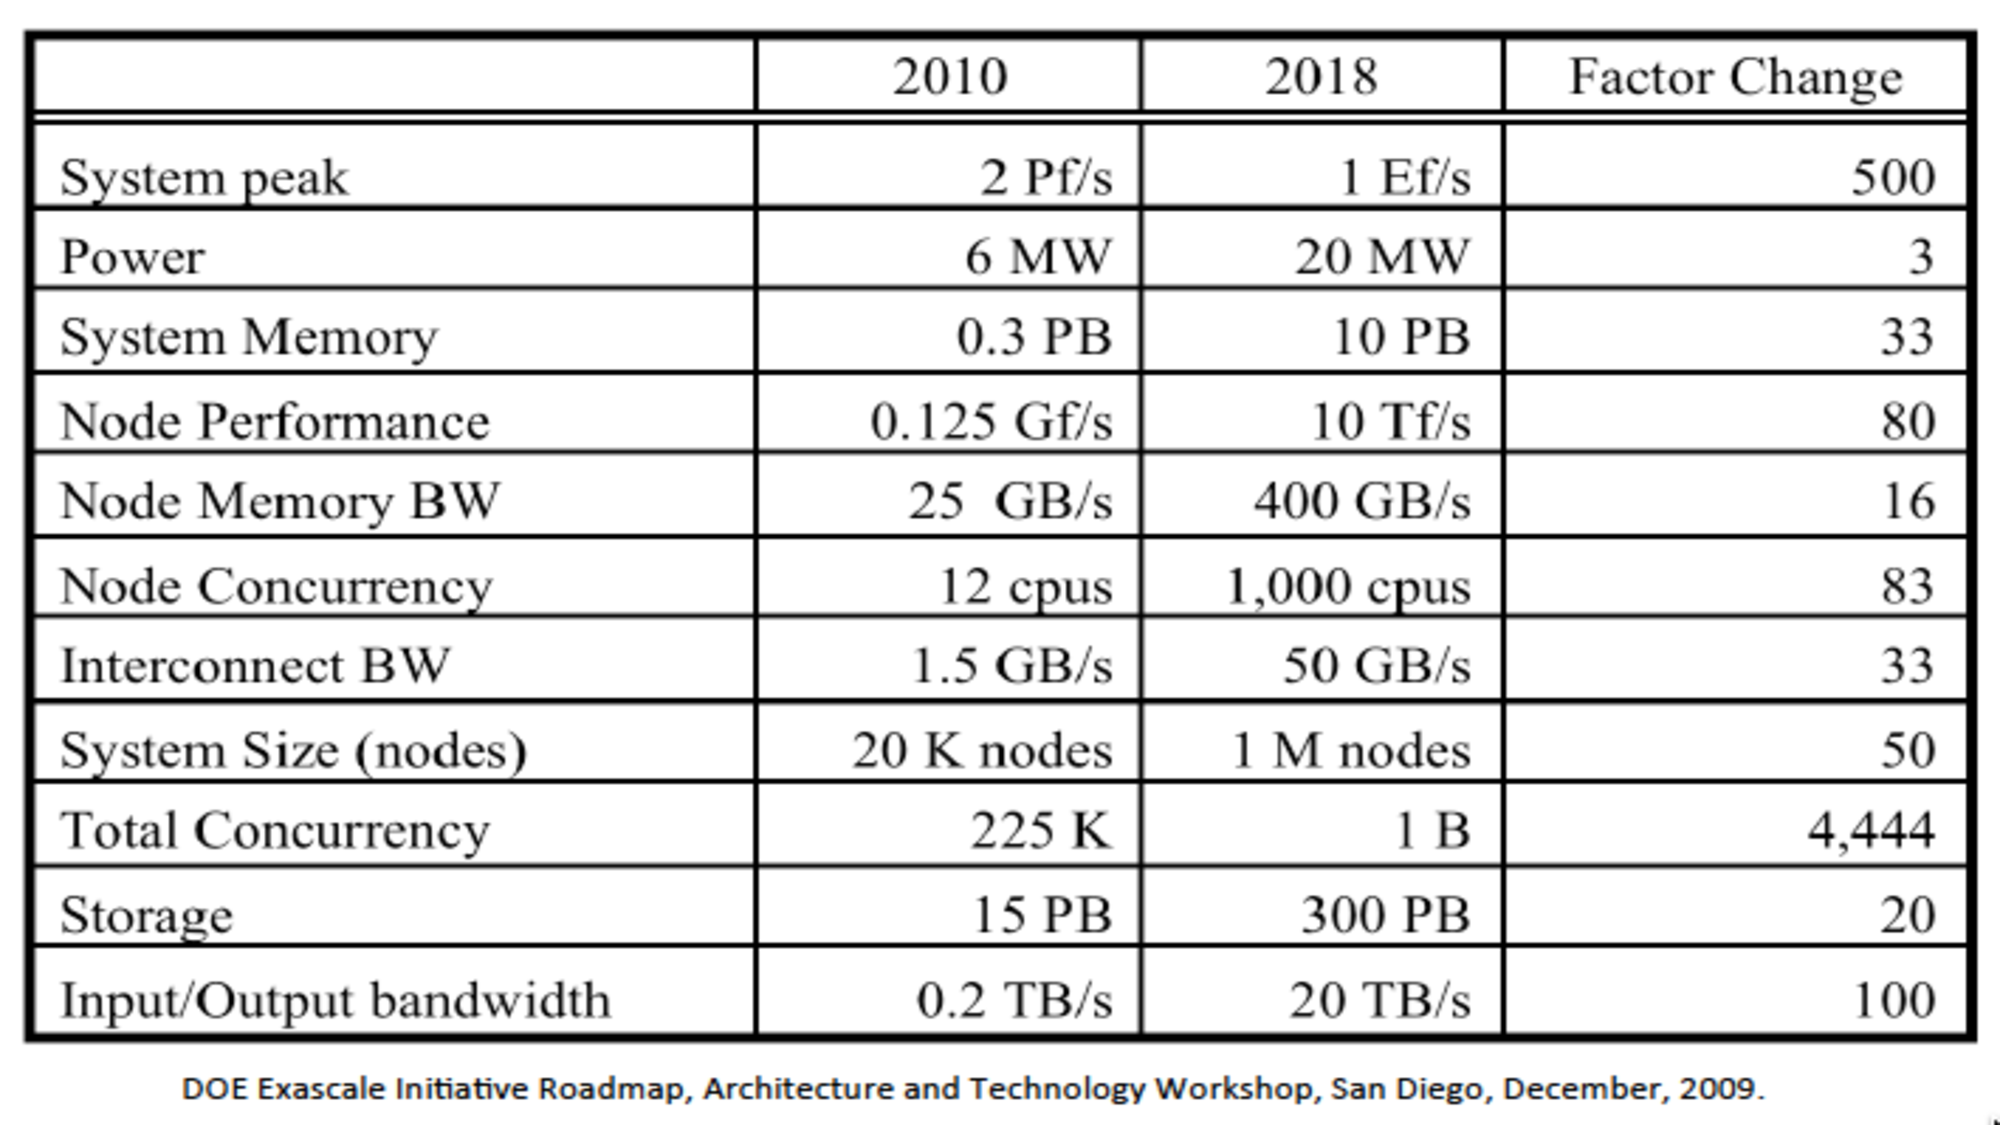
\includegraphics[width=0.85\textwidth]{chapter_1_figures/petascale_to_exascale_chart.pdf}
%    \caption{Concurrency trends in high performance computing
%      platforms.}
%    \label{fig:trends}
%\end{figure}

From the perspective of reproducibility of applications, the trade-off
between performance and determinism presents two distinct
challenges. First, permitting non-deterministic ordering of
interprocess communication opens the door to numerical
irreproducibility via the interaction between reduction order and the
non-associativity of floating-point arithmetic. This is
defined in this thesis as the numerical challenge.

Second, non-determinism significantly hampers debugging efforts during
application development and scaling. Specifically, there exist cases
where bugs manifest only during some executions due to a particular
ordering of message receives. If the application does not guarantee a
specific message receive order then this class of bugs becomes very
hard to diagnose and treat since the cost of reproducing them
significantly increases. Recent work by 
Sato \textit{et. al}~\cite{NINJA:Sato:2017}, 
presents a case-study of the impact of a
non-deterministic bug in terms of developer time and computational
resources. This is defined in this thesis as the debugging challenge.

% Factors that impacts non-determinism associated to the increase
% concurrency include overlapping communication and computation, network
% and configurations delays, and congestion and
% contention. Non-determinism can be internal or external: the first is
% when internal states of the system varies from run to run, and the
% second is when numerical outputs observed vary from run to run.
% Non-determinism is causing two major challenges for the scientific
% community: the numerical and debugging challenges. In numerical
% scenarios, non-determinism does not allow us to control variability
% thresholds (error) in computational results.  In debugging scenarios,
% non-determinism does not allow us to control the interactions among
% processes threads and isolate the causes of rare bugs in software.

\subsection{Overview of Numerical Challenge} 

Because floating-point numbers have finite precision, no simulation
can be completely free of error. As hardware resources grow, the
scientific computation taking advantage of that hardware has become
increasingly complex. A consequence of the scale of computation is
that even small errors at the beginning of the simulation may
eventually compound into significant accuracy problems, which may call
into question the validity of hours and hours of
computation. Multithreading complicates matters by introducing
nondeterminism. Not only do errors accumulate throughout a
computation, but a scientist may run the same computation several
times with differing results. According to a recent report from the
Department of Energy~\cite{Doe2014}, by the end of this decade the
level of concurrency of the supercomputing platforms on which
simulations are executed is expected to increase by a factor of at
least 4000.  The question that must be answered is: Can the scientific
community trust simulations executed on next-generation exascale
architectures?

In Chapter~\ref{chap2}, we assess the effectiveness of several mathematical
techniques to pursue reproducible accuracy on exascale platforms with
multithreading hardware consisting of multicore processors coupled
with many-core accelerators.  We refer to \textit{reproducibility} as
``closeness of agreement among repeated simulation results under the
same initial conditions'' and \textit{accuracy} as ``conformity of a
resulting value to an accepted standard, or scientific laws'' (from
Van Nostrand’s Scientific Encyclopedia). Rather than focusing on
bitwise reproducibility, we study methodologies to minimize the
propagation of errors and, thereby, limit their impact on the results
of a simulation, increasing both the reproducibility of the simulation
and the meaningfulness of the results. 

\subsection{Overview of the Debugging Challenge}

Application developers employ a variety of programming techniques to
maximize the scalability of their applications on the increasingly
concurrent platforms. In the case of message-passing applications, one
notable technique is the use of non-blocking point-to-point
communication, which permits communication and computation to be
overlapped, leading to an increase in scalability. The price paid
however, is the loss of determinism mentioned above. The program's
interprocess communication does not behave exactly the same way during
each execution. Figure~\ref{fig:example_nondeterminism} shows two high
level examples of non-deterministic executions when the same
destinations received the messages in different orders and when
messages are exchanged between two different destinations.
\begin{figure}[!htb]
    \centering
    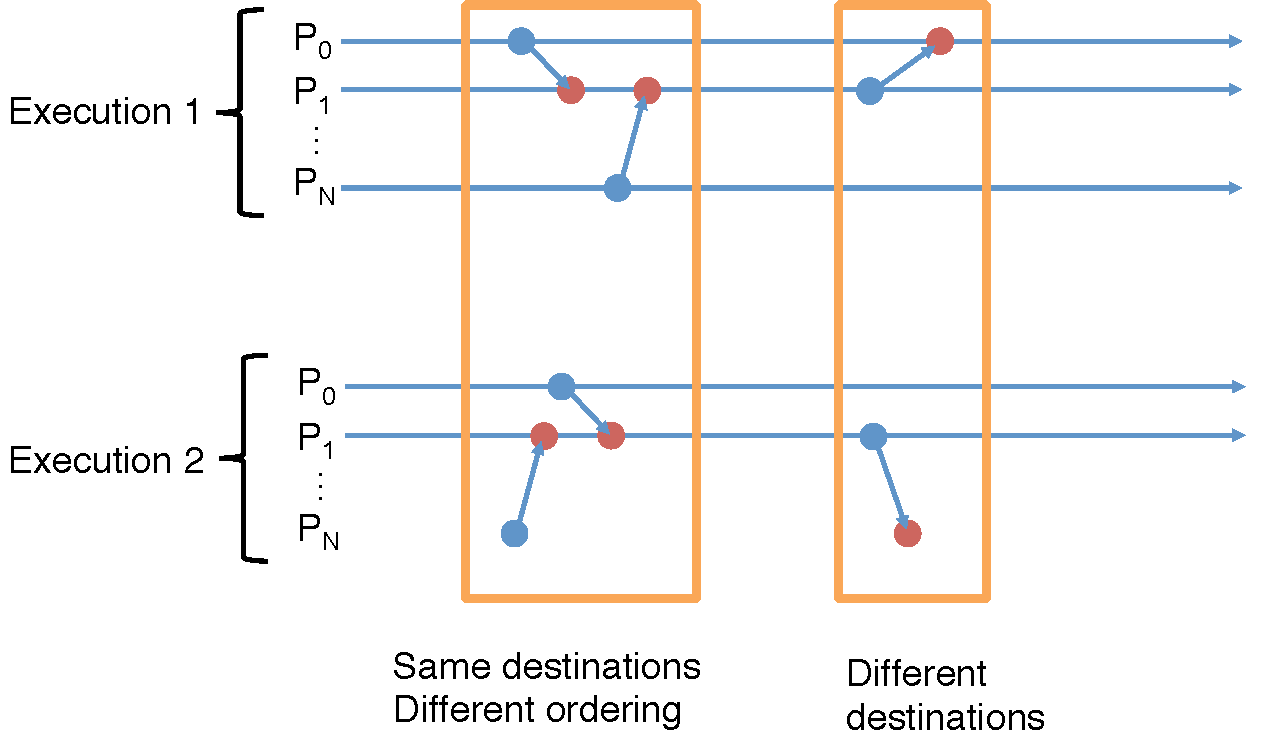
\includegraphics[width=0.85\textwidth]{chapter_1_figures/example_nondeterminism.pdf}
    \caption{Two examples of non-determinism associated to message
      passing executions.}
    \label{fig:example_nondeterminism}
\end{figure}
This problem is further exacerbated by use of wildcard receives (i.e.,
permitting a process to receive its next message from any available
sender, rather than a specific one). This non-determinism impedes
debugging efforts by vastly increasing the cost in computational resources
and developer time needed to reproduce bugs, necessitating the 
use of record-and-replay tools.
The question we address is: How can record-and-replay 
tools be improved so that they can continue to enable debugging on  
future exascale systems. 

In Chapter~\ref{chap3}, we assess the effectiveness of multiple logical
clock ticking policies, including a novel ticking policy we develop,
when used as the underlying ordering mechanism in
Clock-Delta Compression (CDC), a state-of-the-art record-and-replay technique. 
We evaluate ticking policies' effectiveness in enabling CDC's compression
against a real application in a diverse set of runtime conditions that 
reflect variability in floating-point workload and communication intensity 
that HPC applications exhibit. 

\section{Thesis Statement}
We claim that the massive increase in total system concurrency that will accompany 
exascale systems will significantly amplify the problems of numerical
irreproducibility and impededed debugging that HPC developers currently
face. We address the numerical challenge of reproducibility by illustrating
the pressing need for intelligent runtime selection of reduction operators 
for problematic floating-point inputs. We address the debugging challenge 
by demonstrating the pressing need for logical clock ticking policies that 
reduce then out-of-order message rate of the Clock-Delta Compression
record-and-replay technique. 

\section{Contributions}

When dealing with the numerical challenge, our contributions are as
follows:
\begin{itemize}
\item We evaluate and compare the reproducibility of four summation
  techniques applied to a simulated exascale environment.
\item We demonstrate that commonly accepted practices for predicting
  and mitigating errors offer incomplete characterizations of the
  reproducibility of numerical algorithms when applied in isolation.
\item We demonstrate the need for data-aware software to intelligently
  choose reduction algorithms to guarantee reproducibility without an
  unnecessary loss in performance.
\end{itemize}

When dealing with the debugging challenge, our contributions are as
follows:
\begin{itemize}
\item We propose a logical clock ticking policy based on floating-point
    operations that can be integrated in Clock-Delta Compression.
\item We provide a comparison of three ticking policies' 
    (basic Lamport clock ticking, wall-time-based ticking, and FLOPs-based ticking)
    effectiveness under diverse runtime conditions. 
\item We demonstrate the potential for extending logical clock ticking
    policies to adapt to applications' non-deterministic communication patterns.
\end{itemize}

\section{Thesis Outline}
Chapter~\ref{chap2} introduces our work on reproducible numerical
accuracy, and presents results on selection of compensated summation
algorithms based on mathematical properties of summands. Chapter~\ref{chap3}
introduces our work on record-and-replay tools, and presents results 
on our fine-grained logical clock ticking policy as applied to the
Clock-Delta Compression record-and-replay technique. Chapter~\ref{chap4}
lays out the plan for extending our research on reproducibility in HPC
by applying the lessons learned in Chapter~\ref{chap2} and Chapter~\ref{chap3}
to non-deterministic commmunication patterns extracted from applications. 
 
